\documentclass[compress]{beamer}
\usepackage{ifthen}

\title{Summary of the \\ First DT-CSC Joint Alignment Meeting \\ and \\ Alignment Progress Report}
\author{Jim Pivarski}
\institute{Texas A\&M University}
\date{22 March, 2007}

\setbeamertemplate{navigation symbols}{}
\setbeamertemplate{headline}{\includegraphics[height=1 cm]{../cmslogo} \hspace{0.1 cm} \includegraphics[height=1 cm]{../tamulogo} \hfill
\begin{minipage}{9 cm}
\vspace{-0.75 cm} \small
\begin{center}
\ifthenelse{\equal{\insertpagenumber}{1}}{}{\insertsection}
\end{center}
\end{minipage} \hfill
\begin{minipage}{1 cm}
\vspace{-0.75 cm} \small
\begin{center}
\ifthenelse{\equal{\insertpagenumber}{1}}{}{\insertpagenumber/\pageref{numpages}}
\end{center}
\end{minipage}}

%% \xdefinecolor{verylightgray}{rgb}{0.95,0.95,0.95}
%% \beamertemplateshadingbackground{verylightgray}{white}

\xdefinecolor{dkblue}{rgb}{0.1,0.1,0.7}

\begin{document}
\frame{\titlepage}
\section*{Outline --- Jim Pivarski}

\begin{frame}
\frametitle{Two Topics}

\begin{itemize}\setlength{\itemsep}{0.5 cm}
\item Joint Meeting: barrel (Mattoras, Fernandez, Martinez)

\vspace{0.125 cm}
 and endcap (Safonov, Pivarski, Yakorev, Kamon)

\vspace{0.125 cm}
\begin{itemize}\setlength{\itemsep}{0.125 cm}
\item Definition of alignment stream: converging fast
\item Monitoring: largely overlapping ideas \includegraphics[width=0.5 cm]{overlap.png}
\end{itemize}

\item Our alignment progress

\vspace{0.125 cm}
\begin{itemize}\setlength{\itemsep}{0.125 cm}
\item Geometry-comparison tool
\item Layer-by-layer corrections $\to$ DB
\item Stereo DT problem in track-based alignment
\item Survey constraints in alignment framework
\end{itemize}
\end{itemize}
\vfill
\end{frame}

\section*{Definition of alignment stream --- Jim Pivarski}

\begin{frame}
\includegraphics[width=\linewidth]{javier}
\end{frame}

\begin{frame}
\frametitle{Biggest dependency to be avoided: SiClusters}
\begin{itemize}\setlength{\itemsep}{0.5 cm}
\item Included to allow globalMuon track refitting
\begin{itemize}
\item Essential for iterating with tracker-fit tracks (or partly tracker-fit tracks) $\ddot{\smile}$
\item These are low-level tracker hits, and {\it all} of them $\ddot{\frown}$
\end{itemize}
\item Dropping it would cut the file size in half
\item Dependency is due to a hit-cloning operation deep in KFFitter
\item We should somehow remove this dependency \\ (we'll bring it up at AlCaReco meeting tomorrow)
\end{itemize}
\vfill
\end{frame}

\section*{Alignment Monitoring --- Jim Pivarski}

\begin{frame}
\frametitle{Alignment monitoring: roughly four categories}
\begin{enumerate}\setlength{\itemsep}{0.4 cm}
\item DQM-based monitoring upstream of alignment process (reports an error if alignment used online is wrong)
\item Sanity checks in AlignmentProducer (convergence, improvement in residuals, overlap plots, $p_T$)
\item Geometry Validation--- compare output geometries from different alignments: have the chambers moved?
\item Validation with reconstructed tracks: is it better? \\ (same plots as \textcolor{dkblue}{1}?)
\end{enumerate}

\vfill Proposals by barrel, software group differ by merging
\textcolor{dkblue}{3} and \textcolor{dkblue}{4}, whether
\textcolor{dkblue}{2} is a part of AlignmentProducer
\end{frame}

\begin{frame}
\frametitle{Sharing workload}
\begin{enumerate}\setlength{\itemsep}{0.5 cm}
\item DQM-based online monitoring \hfill \textcolor{dkblue}{Javier Fernandez?}
\item Sanity checks in AlignmentProducer \hfill \textcolor{dkblue}{Jim Pivarski?}
\item Geometry Validation \hfill \textcolor{dkblue}{Dmitry Yakorev, Jim Pivarski}
\item Validation with reconstructed tracks \hfill \textcolor{dkblue}{Javier Fernandez?}
\end{enumerate}

\vfill Still under discussion\ldots
\end{frame}

\section*{Alignment Progress --- Jim Pivarski}

\begin{frame}
\frametitle{Next topic: Our alignment progress}

\begin{itemize}\setlength{\itemsep}{0.5 cm}
\item Beginnings of a geometry-comparison tool
\item Working on FAST layer-by-layer corrections $\to$ DB

\vspace{0.25 cm}
(with Karoly and Andrey) 
\item Stereo DT problem in track-based alignment understood, \\ soon to be fixed
\item Survey constraints implemented in alignment framework
\end{itemize}
\end{frame}

\begin{frame}
\frametitle{Geometry-comparison tool (Dmitry Yakorev)}
\begin{columns}
\column{0.03\linewidth}
vs.\ $R$ \\

\vspace{1 cm}
vs.\ $\phi$ \\

\vspace{1 cm}
vs.\ $Z$ \\
\column{0.98\linewidth}
\includegraphics[width=\linewidth]{screen_shot.png}
\end{columns}

\vfill
\hfill $(\vec{x_1}-\vec{x_2})$ \hfill $(\vec{x_1}-\vec{x_2})\cdot\hat{\phi}$ \hfill $(\vec{x_1}-\vec{x_2})\cdot\hat{Z}$ \hfill
\end{frame}

\begin{frame}
\frametitle{Layer-by-Layer corrections}
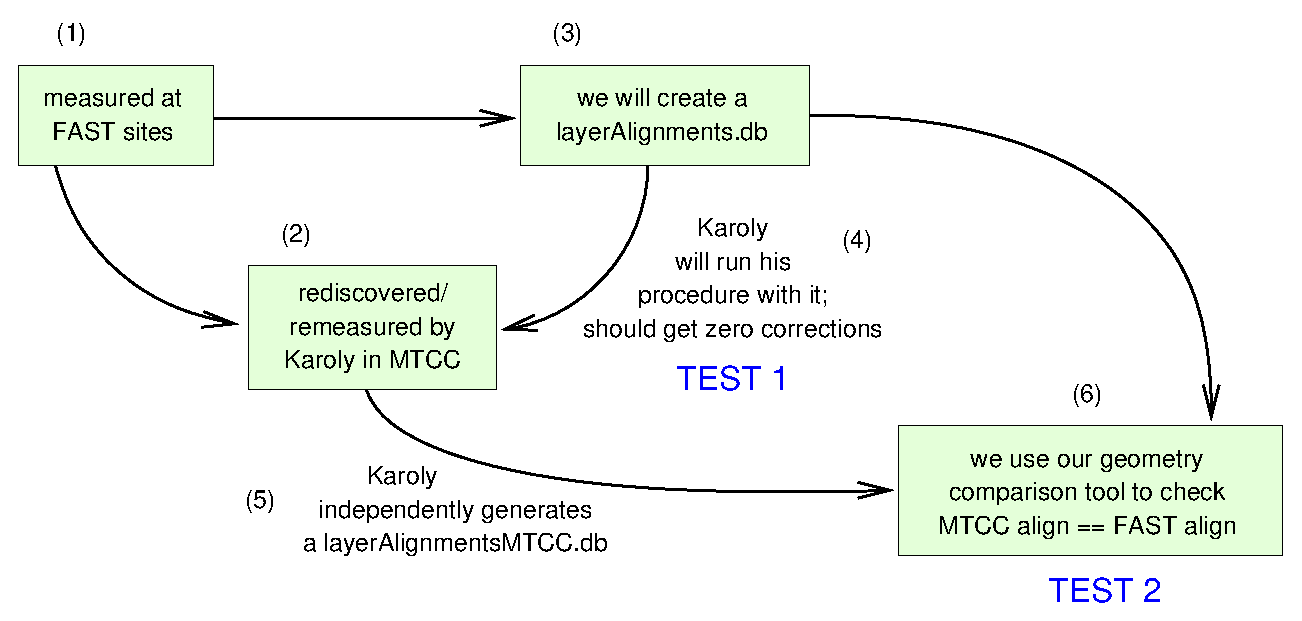
\includegraphics[width=\linewidth]{layerbylayers}

\vfill
\begin{itemize}
\item \textcolor{blue}{TEST 1} is an extension of Karoly's work to all chambers
\item \textcolor{blue}{TEST 2} should be equivalent, and will stress the geometry comparison tool
\end{itemize}
\end{frame}

\begin{frame}
\frametitle{Stereo DT problem in track-based alignment}
This is the only known error in muon alignment procedure in CVS

\vfill What works:
\begin{itemize}
\item DT stereo angle (90$^\circ$) is correctly represented by a rotated local coordinate system (local $y$ is always parallel to wire)
\item ``Meaningful'' residuals ($x_{\mbox{\scriptsize track}} - x_{\mbox{\scriptsize hit}}$) move chambers in the correct directions
\end{itemize}
\vfill What doesn't:
\begin{itemize}
\item ``Meaningless'' residuals ($y_{\mbox{\scriptsize track}} - y_{\mbox{\scriptsize wire midpoint}}$) move chambers
\end{itemize}

\vfill We need to set $1/\sigma^2_{yy}$ to zero, as I did in private code

\vspace{0.125 cm}
Coordinating with tracker alignment to put this in
\end{frame}

\begin{frame}
\frametitle{Survey constraints}
\begin{itemize}\setlength{\itemsep}{0.75 cm}
\item Successfully implemented in tracker alignment
\item We should be able to inherit this work in muon alignment
\item We'll make sure the interface works--- who will apply and check the constraints?
\end{itemize}
\vfill
\end{frame}

\begin{frame}
\frametitle{Recap}
\begin{itemize}\setlength{\itemsep}{0.5 cm}
\item Joint DT/CSC Alignment Meeting

\vspace{0.125 cm}
\begin{itemize}\setlength{\itemsep}{0.125 cm}
\item Definition of alignment stream: converging fast
\item Monitoring: largely overlapping ideas \includegraphics[width=0.5 cm]{overlap.png}
\end{itemize}

\item Alignment progress

\vspace{0.125 cm}
\begin{itemize}\setlength{\itemsep}{0.125 cm}
\item Beginnings of a geometry-comparison tool
\item Working on FAST layer-by-layer corrections $\to$ DB
\item Stereo DT problem in track-based alignment understood, \\ soon to be fixed
\item Survey constraints implemented in alignment framework
\end{itemize}
\end{itemize}
\label{numpages}
\vfill
\end{frame}

\end{document}
